\chapter{Building a Hidden Markov Model for Isolated Signs}
\ifpdf
    \graphicspath{{Chapter2/Chapter2Figs/PNG/}{Chapter2/Chapter2Figs/PDF/}{Chapter2/Chapter2Figs/}}
\else
    \graphicspath{{Chapter2/Chapter2Figs/EPS/}{Chapter2/Chapter2Figs/}}
\fi
% ------------------------------------------------------------------------

\section{Scaling}
In the previous section we introduced methods for solving the evaluation and re-estimation problems for hidden markov models. These methods, whilst mathematically sound, introduce certain problems during implementation. In particular these solutions involve the products of a large number of probabilities, especially for long observation sequence. As a consequence when implemented these methods can cause errors due to underflow. To solve this problem we instead scale the intermediate $\alpha$, $\beta$ and $\gamma$ variables to prevent underflow in the intermediate calculations and choose to compute the logarithm of the probability in the evaluation problem. To do this we normalize the $\alpha_t(i)$ by setting
\begin{align*}
\overline{\alpha}_0(i) = \alpha_0(i) \text{ for each $0\leq i<N$} 
\end{align*}
and inductively defining for each $0\leq t < T$
\begin{align*}
c_t &= \frac{1}{\sum_{i=0}^{N-1}\overline{\alpha}_t(i)}\\
\hat{\alpha}_t(i) &= c_t\overline{\alpha}_t(i)\text{ for each $i$}\\
\overline{\alpha}_{t+1}(i) &= \sum_{i=0}^{N-1}\hat{\alpha}_t(i)a_{ij}b_j(O_{t+1}) \text{ for each $i$}\\
\end{align*}
We then have
\begin{align*}
1 = \sum_{i=0}^{N}\hat{\alpha}_{T-1}(i) &= c_0c_1\dots c_{T-1}\sum_{i=0}^{N}\alpha_{T-i}(j)\\
&=c_0c_1\dots c_{T-1}\mathbb{P}(\mathbf{O}|\lambda)\\
\end{align*}
and hence we can compute the log-probability of an observation sequence $\mathbf{O}$ by
\begin{equation*}
log(\mathbb{P}[\mathbf{O}|\lambda]) = -\sum_{t=0}^{T-1}log(c_t)
\end{equation*}
which allows us to determine probabilities which otherwise would be lost due to underflow. 

Further we can use the same scale factors on the $\beta$ variables as by inductively defining
\begin{align*}
\overline{\beta}_{T-1}(i) &= \beta_{T-1}(i) \\
\hat{\beta}_{t}(i) &= c_t\overline{\beta}_t(i)\\
\overline{\beta}_{t+1}(i) &= \sum_{j=0}^{N-1}a_{ij}b_j(\mathbf{O}_{t+1})\hat{\beta}_{t+1}(i)
\end{align*}
and redefining the $\gamma$ variables as
\begin{align*}
\gamma_t(i,j)&=\hat{\alpha}(i)a_{ij}b_j(\mathbf{O}_{t+1})\beta_{t+1}(j)\\
\gamma_t(i) &= \hat{\alpha}_t(i)\hat{\beta}_t(i)\frac{1}{c_t}
\end{align*}
It has been shown that using these variables in the re-estimation process still ensures that the the probability $\mathbb{P}[\mathbf{O}|\lambda]$ increases with each iteration. 

Using these methods we implemented a general purpose discrete hidden markov model class which can be instantiated with any number with any number of states, observation symbols and probabilities and trained from a collection of observation sequences.
\section{Observation Vector Quantization}

In order to use discrete observation hidden markov models for the problem of gesture recognition we must restrict the continuous observation space to a discrete set of observation symbols. This set of symbols should not be too large (say no more than 30 symbols) to ensure that the problems of training and evaluation can be solved quickly enough for use in a real-time recognition system. Further, an increase in the number of symbols will cause a decrease in the evaluated probability of a given observation sequence being generated by some HMM. If the symbol count is too high this can cause underflow in spite of the effects of scaling. Of course the symbol set should not be too small either as otherwise we might lose some subtle aspects of signs and cause similar signs to be indistinguishable.

To quantize our training data for a single sign we merged all of the points  into a single 3D point cloud and partitioned this point cloud into $k$ clusters. To do this we implemented Lloyd's algorithm to solve the k-means clustering problem. Then for any point we can assign an observation symbol in the range $\{1,\dots,k+1\}$ by taking the number of the cluster with the centroid closest (via Euclidean distance) to the point, or if the distance from the point to each of the means exceeds some threshold assigning the symbol $k+1$. 

\begin{figure}
        \centering
        \begin{subfigure}[b]{0.3\textwidth}
                \centering
                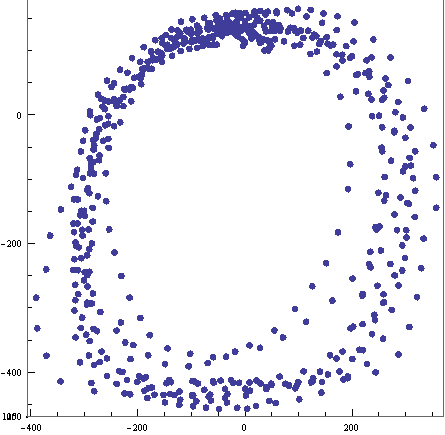
\includegraphics[width=\textwidth]{ThesisFigs/unclusteredCircleGesture}
                \caption{Unclustered circle gesture training data (x-y plane projection)}
                \label{fig:unclust}
        \end{subfigure} 
        \begin{subfigure}[b]{0.3\textwidth}
                \centering
                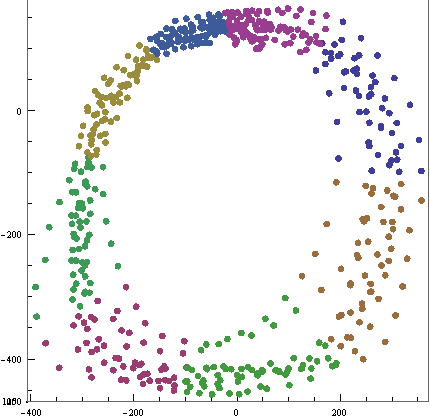
\includegraphics[width=\textwidth]{ThesisFigs/clusteredCircleGesture}
                \caption{Clustered circle gesture training data (x-y plane projection)}
                \label{fig:clust}
        \end{subfigure}
        \caption{The K-Means method for vector quantization}\label{fig:kmeans}
\end{figure}

\subsection{Determining The Initial Topology and Parameters}
As our training method utilises a local search to improve our parameterisation its effectiveness will greatly depend on how we initialise our Hidden Markov Model. If the initial parameterisation is poor then even with a large training set we may fail to find a parameterisation which allows us to  recognise signs with high enough accuracy.

It has been shown that the topology of the underlying Markov Chain can greatly impact the effectiveness of a HMM for a given pattern recognition task~\citep{rabiner1989tutorial, jelinek1998statistical}. The two most common types of HMM are the \emph{ergodic model}, in which each state can transition to any other state in a finite number of steps and the \emph{left-right model} or Bakis model~\citep{bakis1976continuous} in which the state sequence is a (non-strictly) increasing. The left-right model can be viewed as modelling a signal which changes through time, with each transition representing a movement forward in time. For that reason it is more suitable for modelling gestures or speech than other Markov Chain topologies. 

A left-right topology Markov chain is characterized by an upper triangular stochastic matrix $A$. We can further restrict our model to only allow jumps from a state $i$ to states $i \leq j \leq j+\Delta$ for some $\Delta$. This restriction can prevent the model being pushed, through re-parameterisation, into a trivial Markov chain which remains at the final state $N$ at all times. This can be seen as imposing a restriction on the velocity we can expect a signer's hand to move at - not allowing him to pass by too many states in quick succession.

As such we choose to intialize our HMMs as left-right models restricted to $\Delta = 1$. Hence we initialise the stochastic matrix with form
\begin{equation*}
A =
 \begin{pmatrix}
  a_{11} & a_{12} & 0 & \cdots & 0 \\
  0 & a_{22} & a_{23} &\cdots & 0 \\
  \vdots  & \vdots  & \vdots & \ddots & \vdots  \\
  0 & 0 & \cdots & a_{(n-1)(n-1)}& a_{(n-1)n} \\
  0 & 0 & \cdots & 0& 1
 \end{pmatrix}
\end{equation*}
and define $\pi = [1,0, \dots, 0]$. Clearly if we initialise the non-zero $a_{ij}$ of A deterministically then we restrict ourselves to single outcome from the re-estimation procedure, as such we choose to introduce some randomness in the stochastic matrix when it is initialized. Setting
\begin{align*}
&a_{ii} = 0.5 - r &a_{i(i+1)} = 0.5 + r
\end{align*}
 for some $r$ chose uniformly from the interval $[-0.3, +0.3]$, which is chosed to ensure that none of the links are set too weakly and the forward transitions broken during re-estimation.

As we expect the system to differentiate a large number of signs it would be a major task to taylor the initialistions of each Hidden Markov Model to the sign it is expected to recognise. Hence, we choose to use the same initial estimation procedure for each HMM and do not make any inferences about the structure of the emissions matrix $B$ given the sign it is expected model.
% ------------------------------------------------------------------------

%%% Local Variables: 
%%% mode: latex
%%% TeX-master: "../thesis"
%%% End: 
